% Options for packages loaded elsewhere
\PassOptionsToPackage{unicode}{hyperref}
\PassOptionsToPackage{hyphens}{url}
\documentclass[
]{article}
\usepackage{xcolor}
\usepackage[margin=24mm]{geometry}
\usepackage{amsmath,amssymb}
\setcounter{secnumdepth}{-\maxdimen} % remove section numbering
\usepackage{iftex}
\ifPDFTeX
  \usepackage[T1]{fontenc}
  \usepackage[utf8]{inputenc}
  \usepackage{textcomp} % provide euro and other symbols
\else % if luatex or xetex
  \usepackage{unicode-math} % this also loads fontspec
  \defaultfontfeatures{Scale=MatchLowercase}
  \defaultfontfeatures[\rmfamily]{Ligatures=TeX,Scale=1}
\fi
\usepackage{lmodern}
\ifPDFTeX\else
  % xetex/luatex font selection
\fi
% Use upquote if available, for straight quotes in verbatim environments
\IfFileExists{upquote.sty}{\usepackage{upquote}}{}
\IfFileExists{microtype.sty}{% use microtype if available
  \usepackage[]{microtype}
  \UseMicrotypeSet[protrusion]{basicmath} % disable protrusion for tt fonts
}{}
\makeatletter
\@ifundefined{KOMAClassName}{% if non-KOMA class
  \IfFileExists{parskip.sty}{%
    \usepackage{parskip}
  }{% else
    \setlength{\parindent}{0pt}
    \setlength{\parskip}{6pt plus 2pt minus 1pt}}
}{% if KOMA class
  \KOMAoptions{parskip=half}}
\makeatother
\usepackage{graphicx}
\makeatletter
\newsavebox\pandoc@box
\newcommand*\pandocbounded[1]{% scales image to fit in text height/width
  \sbox\pandoc@box{#1}%
  \Gscale@div\@tempa{\textheight}{\dimexpr\ht\pandoc@box+\dp\pandoc@box\relax}%
  \Gscale@div\@tempb{\linewidth}{\wd\pandoc@box}%
  \ifdim\@tempb\p@<\@tempa\p@\let\@tempa\@tempb\fi% select the smaller of both
  \ifdim\@tempa\p@<\p@\scalebox{\@tempa}{\usebox\pandoc@box}%
  \else\usebox{\pandoc@box}%
  \fi%
}
% Set default figure placement to htbp
\def\fps@figure{htbp}
\makeatother
\setlength{\emergencystretch}{3em} % prevent overfull lines
\providecommand{\tightlist}{%
  \setlength{\itemsep}{0pt}\setlength{\parskip}{0pt}}
\usepackage{mathrsfs}
\usepackage{mathtools}
\DeclareUnicodeCharacter{2212}{\ensuremath{-}}

\DeclareUnicodeCharacter{2265}{\ensuremath{\ge}}
\DeclareUnicodeCharacter{2264}{\ensuremath{\le}}
\DeclareUnicodeCharacter{2295}{\ensuremath{\oplus}}
\DeclareUnicodeCharacter{2297}{\ensuremath{\otimes}}
\DeclareUnicodeCharacter{2208}{\ensuremath{\in}}
\DeclareUnicodeCharacter{2261}{\ensuremath{\equiv}}
\DeclareUnicodeCharacter{21A6}{\ensuremath{\mapsto}}
\DeclareUnicodeCharacter{2192}{\ensuremath{\to}}
\DeclareUnicodeCharacter{03BA}{\ensuremath{\kappa}}
\DeclareUnicodeCharacter{039B}{\ensuremath{\Lambda}}
\DeclareUnicodeCharacter{03C4}{\ensuremath{\tau}}
\DeclareUnicodeCharacter{03A9}{\ensuremath{\Omega}}
\usepackage{bookmark}
\IfFileExists{xurl.sty}{\usepackage{xurl}}{} % add URL line breaks if available
\urlstyle{same}
\hypersetup{
  hidelinks,
  pdfcreator={LaTeX via pandoc}}

\author{}
\date{}

\begin{document}

{
\setcounter{tocdepth}{3}
\tableofcontents
}
\section{Observed support at the shifted nilpotent
collision}\label{observed-support-at-the-shifted-nilpotent-collision}

This note constructs the full support-algebra receiver at the observed
collision, identifies its restriction-of-scalars defect with the kernel
of the original observed current, and transports sharp signed current
bounds through the exact rank-one correction. The original observation,
its metric, the selfadjoint part of the arithmetic operator, and the
measured support weights remain in the comparison.

The source inputs are
\href{https://github.com/KokunoYumeto/zeta-function-research-reader/blob/4ba9285b66af58a6d58fc502a494c1fb45ca5b79/workbenches/splitzero-tandem/continuations/20260922-support-transport/SUPPORT_SPECTRUM_AND_TERMINAL_MASS.md}{\emph{What
the original observation retains of split support}, ST1--ST20},
\href{https://github.com/KokunoYumeto/zeta-function-research-reader/blob/4ba9285b66af58a6d58fc502a494c1fb45ca5b79/workbenches/splitzero-tandem/continuations/20260922-support-transport/OBSERVED_DEFORMATION_AND_CURRENT.md}{\emph{The
support deformation after the original observation}, DF1--DF16}, and
\href{https://github.com/KokunoYumeto/zeta-function-research-reader/blob/6af54ea3c8ef99127af327f3103e086c68d482c2/workbenches/splitzero-tandem/branches/identity-absorber-square/NATIVE_DUAL_NUMBER_RECEIVER.md}{\emph{The
standard dual-number infinitesimal in the original arithmetic action},
NI1--NI29}. Those complete notes were read. The dimension proof
additionally uses OCP11--OCP12 in
\href{https://github.com/KokunoYumeto/zeta-function-research-reader/blob/6af54ea3c8ef99127af327f3103e086c68d482c2/workbenches/splitzero-tandem/branches/identity-absorber-square/sources/OBSERVED_CURRENT_PLANE.tex}{\emph{The
original observed arithmetic-current plane}}, whose original-object and
conductor sections were read. The finite calculations below are proved
in full; no arithmetic asymptotic theorem is reproved here.

\subsection{1. The actual observed dimension and the retained
metric}\label{the-actual-observed-dimension-and-the-retained-metric}

At every original cutoff \(q-1\le N\le2q\), keep \[
k\ge17,\quad k\equiv1\pmod4,\quad q=(k+1)^2,
\quad q_0=(k-7)^2,\quad \Delta_0=q-q_0=16k-48.
\tag{OSP1}
\] The source is \(E=\mathbb C[y]/Q_k\), with the original onto
observation \(\Lambda:E\to B\), complete metric, and section \[
Q_B=(\Lambda G_N^{-1}\Lambda^*)^{-1},\quad
L=G_N^{-1}\Lambda^*Q_B,\quad J=LQ_B^{-1/2},
\quad J^\dagger J=I_B,\quad P_B=JJ^\dagger.
\tag{OSP2}
\] All observed vectors below are in these Euclidean coordinates; the
isometry \(J\) retains their exact original metric. Keep \[
M=C+R,\quad C=C^\dagger,\quad R=\epsilon fe^\dagger,
\quad\|e\|=\|f\|=1,\quad e^\dagger f=0,\quad\epsilon>0.
\tag{OSP3}
\]

The observation has dimension at least \(q_0\). Indeed the original
conductor satisfies \[
C_A:E\to E_0=\mathbb C[y]/Q_{k-8},\quad
C_A[p]=[\mathcal Tp],\quad\ker\Lambda\subseteq\ker C_A.
\tag{OSP4}
\] Its first nonzero moment has order \(v_0\le80\) and coefficient
\(\mu_{v_0}\ne0\). The image of a monic degree-\(n\) polynomial, for
\(n\ge v_0\), has degree \(n-v_0\) and leading coefficient \[
\kappa_n=i^{-v_0}\mu_{v_0}\binom n{v_0}\ne0.
\tag{OSP5}
\] These are OCP11--OCP12, with the original phase retained. Expanding
the finite translated monomials also proves the degree assertion
directly: all smaller moments vanish and the first surviving term has
exactly this coefficient.

For \(j=0,\ldots,q_0-1\), take a monic polynomial of degree \(v_0+j\).
Since \(v_0\le80<\Delta_0\), these degrees are below \(q\). Their
conductor images have successive degrees \(0,\ldots,q_0-1\) with nonzero
leading coefficients. They form a triangular basis of the polynomials of
degree below \(q_0\), hence a basis modulo the monic polynomial
\(Q_{k-8}\). Thus \(C_A\) is onto. The kernel inclusion in (OSP4)
defines an onto map \(\overline C_A:B\to E_0\), by
\(\overline C_A(\Lambda x)=C_Ax\). This is well-defined by that
inclusion. Therefore \[
m:=\dim_{\mathbb C}B\ge q_0\ge100.
\tag{OSP6}
\] In particular the complementary support used below exists on the
actual observation.

\subsection{2. The measured support and its exact range
projector}\label{the-measured-support-and-its-exact-range-projector}

Put \[
u=J^\dagger e,\quad v=J^\dagger f,\quad U=[u,v],\quad
\mathcal C=U^*U=\begin{pmatrix}a&r\\\overline r&d\end{pmatrix},
\quad\mathfrak d=ad-|r|^2,\quad A=UU^*,\quad\alpha=1-a.
\tag{OSP7}
\] The symbol \(\mathfrak d\) is the Gram determinant of ST5 and DF4; it
is the quantity also denoted \(\Delta\) in the collision paper. On the
original finite area guards, \[
0\prec\mathcal C\preceq I_2,\qquad\mathfrak d\ge\Theta_N>0.
\tag{OSP8}
\] The upper inequality follows also because
\((z_1,z_2)\mapsto z_1e+z_2f\) is an isometry and \(J^\dagger\) is a
contraction. The finite lower bound is the original two-column area
input, not a consequence of separate column norms.

Define the exact orthonormal frame and its complementary space by \[
g=u/\sqrt a,\qquad
h=\frac{v-(r/a)u}{\sqrt{\mathfrak d/a}},\quad
S=\operatorname{span}\{g,h\},\quad H=S^\perp.
\tag{OSP9}
\] The numerator defining \(h\) is orthogonal to \(u\) and has squared
norm \(d-|r|^2/a=\mathfrak d/a\). Thus the formula keeps its exact
positive denominator. The range projector is \[
P=U\mathcal C^{-1}U^*=gg^*+hh^*,\qquad\ker P=H.
\tag{OSP10}
\] Multiplication gives \(P^2=P=P^*\) and \(PU=U\), proving this
assertion. The actual measured support has the different matrix \[
A|_S=\begin{pmatrix}
a+|r|^2/a&r\sqrt{\mathfrak d}/a\\
\overline r\sqrt{\mathfrak d}/a&\mathfrak d/a
\end{pmatrix},\qquad A|_H=0.
\tag{OSP11}
\] This follows by substituting \(u=\sqrt a\,g\) and
\(v=(r/\sqrt a)g+\sqrt{\mathfrak d/a}\,h\) into \(UU^*\).

The two nonzero eigenvalues of \(A\) are \[
\vartheta_\pm=\frac{a+d\pm\sqrt{(a-d)^2+4|r|^2}}2,
\qquad0<\vartheta_-\le\vartheta_+\le1.
\tag{OSP12}
\] Indeed \(A(Uz)=U\mathcal Cz\), and \(U\) is injective. Conversely a
nonzero eigenvector of \(A\) belongs to its range. This identifies the
two nonzero spectra; the quadratic formula proves the display.
Consequently \[
\vartheta_-P\preceq A\preceq\vartheta_+P,\qquad
P=\frac{(a+d)A-A^2}{\mathfrak d},\qquad
\|P-A\|=1-\vartheta_-.
\tag{OSP13}
\] For the middle identity, use
\(\mathcal C^2-(a+d)\mathcal C+\mathfrak dI_2=0\), multiply its
rearrangement by \(U\mathcal C^{-1}\) and \(U^*\), and use (OSP10). The
other assertions follow on the orthonormal eigenbasis of the plane and
the common zero action on \(H\). Also
\(\vartheta_-=\mathfrak d/\vartheta_+\ge\Theta_N\), so
\(a,d\ge\Theta_N\).

With the original source projection \(\Pi=ee^\dagger+ff^\dagger\), the
full measured defect remains \[
A-A^2=D^\dagger D,\qquad D=(I-P_B)\Pi J.
\tag{OSP14}
\] Insert \(P_B=JJ^\dagger\) in \(J^\dagger\Pi^2J-(J^\dagger\Pi J)^2\),
using \(\Pi^2=\Pi\), to obtain this exact identity. Thus recovering
\(P\) from \(A\) does not discard its two measured weights or its
original kernel contribution.

\subsection{3. Collision and the kernel of the original
current}\label{collision-and-the-kernel-of-the-original-current}

Keep the full observed family \[
M_B(s)=C_B+F_B(s),\quad C_B=J^\dagger CJ=C_B^*,\quad
F_B(s)=(\epsilon v+su)u^*,\quad\lambda(s)=as+\epsilon r.
\tag{OSP15}
\] Its native value is \(M_B(0)\). Multiplication gives
\(F_B(s)^2=\lambda(s)F_B(s)\). At the exact collision, \[
s_*=-\epsilon r/a,\quad
N_*=F_B(s_*)=\epsilon vu^*-\frac{\epsilon r}{a}uu^*
=b_0hg^*,\qquad b_0=\epsilon\sqrt{\mathfrak d}>0.
\tag{OSP16}
\] Thus \(N_*g=b_0h\), \(N_*h=0\), \(N_*H=0\), and \(N_*^2=0\). In
particular the collision retains a nonzero operator with the stated area
amplitude.

Write \(\beta=\Im r\); this symbol never denotes the amplitude \(b_0\).
The original and collision currents satisfy \[
W_0=i(M_B(0)-M_B(0)^*)=i\epsilon(vu^*-uv^*),
\] \[
W_*=i(M_B(s_*)-M_B(s_*)^*)=i(N_*-N_*^*)
=W_0+\frac{2\epsilon\beta}{a}uu^*.
\tag{OSP17}
\] Here the same \(C_B\) cancels because it is selfadjoint; it remains
in both full arithmetic operators. In the frame (OSP9), \[
W_0|_S=\begin{pmatrix}-2\epsilon\beta&-ib_0\\ib_0&0\end{pmatrix},
\qquad W_*|_S=\begin{pmatrix}0&-ib_0\\ib_0&0\end{pmatrix}.
\tag{OSP18}
\] Both vanish on \(H\), and both active determinants are
\(-b_0^2=-\epsilon^2\mathfrak d\ne0\). Therefore \[
\ker W_0=\ker W_*=H,\qquad
P=\frac{W_*^2}{\epsilon^2\mathfrak d}
=\frac{W_0^2+2\epsilon\beta W_0}{\epsilon^2\mathfrak d}.
\tag{OSP19}
\] The polynomial formulas follow by multiplying (OSP18) and checking
the common zero action on \(H\). This identifies the original
observed-current kernel exactly, despite the nonzero current correction.

The full operator and current corrections have exact norms \[
M_B(s_*)-M_B(0)=-\frac{\epsilon r}{a}uu^*,\quad
\|M_B(s_*)-M_B(0)\|=\epsilon|r|,
\] \[
W_*-W_0=2\epsilon\beta gg^*,\quad
\|W_*-W_0\|=2\epsilon|\beta|.
\tag{OSP20}
\] These follow from \(\|uu^*\|=a\) and \(\|gg^*\|=1\). Positivity of
\(I-\mathcal C\) gives \(|r|^2\le\alpha(1-d)\le\alpha\). Hence the
finite relative bounds are \[
\frac{\|N_*-F_B(0)\|}{b_0}=\frac{|r|}{\sqrt{\mathfrak d}}
\le\sqrt{\alpha/\Theta_N},\qquad
\frac{\|W_*-W_0\|}{b_0}\le2\sqrt{\alpha/\Theta_N}.
\tag{OSP21}
\] Neither the real nor imaginary part of the original return \(r\) has
been removed.

\subsection{4. Full support and the original-current Tor
space}\label{full-support-and-the-original-current-tor-space}

Put \(D_{\mathbb C}=\mathbb C[\eta]/\eta^2\),
\(Q_{\mathbb C}=\mathbb C\times D_{\mathbb C}\), and \(E_0=(0,1)\).
Define \[
\Sigma_*:Q_{\mathbb C}\hookrightarrow\operatorname{End}_{\mathbb C}(B),
\qquad(z,c+\ell\eta)\longmapsto z(I-P)+cP+\ell N_*.
\tag{OSP22}
\] The identities \(P^2=P\), \(PN_*=N_*P=N_*\), and \(N_*^2=0\) prove
multiplication and the unit formula. For injectivity, apply a zero image
to a nonzero vector of \(H\), then to \(h\), then to \(g\). Since
\(\dim H=m-2\ge98\) and \(b_0>0\), these applications give
\(z=c=\ell=0\).

The original additive-monoid symbols have exact images \[
[\tau]\mapsto I_B,\quad [e]\mapsto P,\quad
[n^\bullet]\mapsto P+nN_*,\quad [1^\bullet]-[e]\mapsto N_*.
\tag{OSP23}
\] Indeed \((P+mN_*)(P+nN_*)=P+(m+n)N_*\), which is the supported
addition law. The additive-monoid ring is
\(\mathbb C\times\mathbb C[t^{\pm1}]\); in its supported corner, \(t\)
maps to \(P+N_*\), with inverse \(P-N_*\). Division by \((t-1)^2\)
leaves a constant and a linear term, whose images \(P,N_*\) are
independent. Thus its kernel is precisely the square of the original
support ideal. The primitive, supported integer zero, and external
identity have their separate stated maps.

There is an exact module decomposition \[
B\cong H\oplus D_{\mathbb C},\quad
(z_0,c+\ell\eta)\longmapsto z_0+cg+\ell b_0h,
\] \[
B\cong((1-E_0)Q_{\mathbb C})^{m-2}\oplus E_0Q_{\mathbb C}.
\tag{OSP24}
\] The first formula is a module map by (OSP22) and bijective by
orthogonal decomposition. A basis of \(H\) gives the second. Both
idempotent modules are direct summands of \(Q_{\mathbb C}\), proving
finite projectivity. The exact metric on the dual-number summand is
\(|c|^2+b_0^2|\ell|^2\).

Restrict scalars along \[
D_{\mathbb C}\hookrightarrow Q_{\mathbb C},\qquad
c+\ell\eta\longmapsto(c,c+\ell\eta).
\tag{OSP25}
\] Then \(\eta\) acts as \(N_*\). The periodic free resolution of
\(\mathbb C=D_{\mathbb C}/\eta D_{\mathbb C}\), with each positive
differential multiplication by \(\eta\), is exact because that
multiplication has both kernel and image \(\eta D_{\mathbb C}\). After
tensoring with \(B\), every differential is \(N_*\). Consequently, for
every \(i\ge1\), \[
\operatorname{Tor}^{D_{\mathbb C}}_i(\mathbb C,B)
=\ker N_*/\operatorname{im}N_*
\xrightarrow{\sim}H=\ker W_0.
\tag{OSP26}
\] The last map takes a class to its unique orthogonal representative in
\(H\), since \(\ker N_*=\mathbb Ch\oplus H\) and
\(\operatorname{im}N_*=\mathbb Ch\). This also proves the
quotient-metric identification. The nonzero Tor space belongs to the
original observed current, while the same underlying observed space is
projective over the full support algebra.

\subsection{5. Cubic roots cross the observed support
sectors}\label{cubic-roots-cross-the-observed-support-sectors}

For every unit vector \(z\in H\), define \[
T_z=\sqrt{b_0}(hz^*+zg^*),\qquad
\sqrt{b_0}=\sqrt\epsilon\,\mathfrak d^{1/4}.
\tag{OSP27}
\] It sends \(g\) to \(\sqrt{b_0}z\), \(z\) to \(\sqrt{b_0}h\), and
\(h\) to zero, and vanishes on their common orthogonal complement.
Therefore \[
T_z^2=N_*,\quad T_z^3=0,\quad
PT_zP=0,\quad (I-P)T_z(I-P)=0.
\tag{OSP28}
\] Its two typed mixed maps are \[
S\xrightarrow{\alpha_z}H\xrightarrow{\beta_z}S,
\quad\alpha_z=\sqrt{b_0}zg^*,\quad
\beta_z=\sqrt{b_0}hz^*,\quad
\beta_z\alpha_z=N_*|_S,\quad\alpha_z\beta_z=0.
\tag{OSP29}
\] The composites follow from \(z^*z=1\) and \(g^*h=0\). The parameter
space is the unit sphere in the actual original-current kernel \(H\); no
particular member is selected.

The entire node thickening has the receiver \[
\mathbb C[t^{\pm1},u^{\pm1}]/((t-1)^2(u-1)^2)
\longrightarrow\mathbb C[T_z],\qquad t,u\longmapsto I+T_z,
\tag{OSP30}
\] with kernel \((t-u,(t-1)^3)\) in the displayed source. The
inverse-variable formula is \((I+T_z)^{-1}=I-T_z+T_z^2\), and
\(j=(t-1)(u-1)\) maps to \(N_*\). Quotienting by the stated kernel gives
\(\mathbb C[x]/x^3\), whose three operator images are independent: apply
a proposed relation successively to \(h,z,g\). This proves the exact
kernel.

The primitive diagonal receiver instead sends \(t,u\) to \(I+N_*\), so
\(t-1\mapsto N_*\) and \(j\mapsto0\). The connecting map
\(\mathbb C[T_z]\to\mathbb C[I,N_*]\), \(T_z\mapsto N_*\), is onto with
kernel \(\mathbb CT_z^2\), by the two polynomial presentations. It is
different from inclusion of operator algebras. Thus the primitive and
smoothing routes, and their actual different images of \(j\), remain
specified.

\subsection{6. The corrected algebra receiver and the original
compression}\label{the-corrected-algebra-receiver-and-the-original-compression}

Let \(\Sigma\) be the original full support receiver in ST4 and
\(\Phi(X)=J^\dagger XJ\) the original observation. Substitution gives \[
\Phi\Sigma(z,c+\ell\eta)=z(I-A)+cA+\ell\epsilon vu^*,
\] \[
\Sigma_*(z,c+\ell\eta)-\Phi\Sigma(z,c+\ell\eta)
=(c-z)(P-A)-\ell\frac{\epsilon r}{a}uu^*.
\tag{OSP31}
\] The first term retains the measured support discrepancy, and the
second retains the complex collision displacement. The compression is
linear and unital; its exact multiplicative defect is \[
\Phi(XY)-\Phi(X)\Phi(Y)=J^\dagger X(I-P_B)YJ.
\tag{OSP32}
\] This follows by inserting \(P_B=JJ^\dagger\) between \(X\) and \(Y\).
Equation (OSP31) therefore compares the actual compressed source map
with the proved collision algebra map, without declaring the compression
multiplicative or deleting either correction.

\subsection{7. Sharp signed bounds using the measured
support}\label{sharp-signed-bounds-using-the-measured-support}

For any \(y_0\in B\), put \(s_A(y_0)=y_0^*Ay_0=\|U^*y_0\|^2\). The
original current has the sharp operator bounds \[
-\epsilon A\preceq W_0\preceq\epsilon A.
\tag{OSP33}
\] Indeed \(W_0=\epsilon UJ_2U^*\), with
\(J_2=\left(\begin{smallmatrix}0&-i\\i&0\end{smallmatrix}\right)\),
whose eigenvalues are \(\pm1\). Apply its quadratic-form bounds to
\(U^*y_0\). Both equalities occur: for \(v_\pm=(1,\pm i)^T\), take
\(y_\pm=U\mathcal C^{-1}v_\pm\), giving \(U^*y_\pm=v_\pm\). Neither
constant can therefore be improved.

The exact rank-one transport preserves the sharp inequalities \[
-\epsilon A+\frac{2\epsilon\beta}{a}uu^*
\preceq W_*\preceq
\epsilon A+\frac{2\epsilon\beta}{a}uu^*.
\tag{OSP34}
\] The same equality probes apply because subtracting the displayed
correction gives exactly \(W_0\). In scalar form, \[
-\epsilon s_A(y_0)+\frac{2\epsilon\beta}{a}|u^*y_0|^2
\le y_0^*W_*y_0\le
\epsilon s_A(y_0)+\frac{2\epsilon\beta}{a}|u^*y_0|^2.
\tag{OSP35}
\] The sign of \(\beta=\Im r\) has not been replaced by its magnitude.

There are also optimal constants for inequalities using only \(A\) on
their right sides. Set \[
\zeta=\frac{\Im r}{a},\qquad
\theta_\pm=\zeta\pm\sqrt{1+\zeta^2}.
\] Then \[
\epsilon\theta_- A\preceq W_*\preceq\epsilon\theta_+ A,
\qquad\theta_-<0<\theta_+,\quad\theta_-\theta_+=-1.
\tag{OSP36}
\] For a proof including sharpness, write \[
W_*=\epsilon U\begin{pmatrix}2\zeta&-i\\i&0\end{pmatrix}U^*.
\] The Hermitian matrix has characteristic polynomial \(z^2-2\zeta z-1\)
and eigenvectors \((\theta_\pm,i)^T\). Its quadratic-form bounds prove
(OSP36). The vectors \(y_\pm=U\mathcal C^{-1}(\theta_\pm,i)^T\) attain
the two equalities. This proves the optimal constants with the actual
measured support, including its generally unequal positive and negative
weights.

The exact orthogonal-support bounds are \[
-b_0P\preceq W_*\preceq b_0P,
\tag{OSP37}
\] with equality on \(g-ih\) and \(g+ih\), respectively. This follows
directly from (OSP18). Their relationship with measured support is the
exact weighted comparison (OSP13), rather than an identification of
\(A\) with \(P\).

\subsection{8. The finite terminal mass
bound}\label{the-finite-terminal-mass-bound}

Retain the exact terminal cardinal and its original domain from ST13:
\(\gamma\ge1000\delta\), the stipulated five-orbit condition, and the
admitted-period guard \(|\varpi|\ge R_{\rm corner}\), which establish
nonzero original observed terminal mass. In the same coordinates put \[
\widehat y=\frac{J^\dagger x_{\rm term}}{\|P_Bx_{\rm term}\|},
\quad\|\widehat y\|=1,\quad
c_g=g^*\widehat y,\quad c_h=h^*\widehat y,
\quad |c_g|\le\eta_N.
\tag{OSP38}
\] Here \(\eta_N\) is the original finite terminal bound in TR10, as
used in ST13. Its arithmetic derivation is not replaced. Define \[
\mu=|c_g|^2+|c_h|^2=\widehat y^*P\widehat y,
\quad\mathfrak s=\widehat y^*A\widehat y,
\quad E_N^{\rm supp}=(\eta_N+\sqrt\alpha)^2.
\tag{OSP39}
\] The exact finite measured-mass estimate is \[
|\mathfrak s-d\mu|\le E_N^{\rm supp},\qquad
\mu_-\le\mu\le\mu_+,
\] \[
\mu_-:=\max\{0,(\mathfrak s-E_N^{\rm supp})/d\},\qquad
\mu_+:=\min\{1,(\mathfrak s+E_N^{\rm supp})/d\}.
\tag{OSP40}
\] For its complete finite proof, subtract \(d\mu\) from (OSP11)'s
quadratic form. The coefficient at \(|c_g|^2\) is \(a+|r|^2/a-d\), of
absolute value at most one: \(\mathcal C^2\preceq\mathcal C\) gives
\(|r|^2/a\le1-a=\alpha\), while \(0<d\le1\). The other diagonal term has
magnitude at most \(\alpha|c_h|^2\le\alpha\). The off-diagonal term has
magnitude at most
\(2\sqrt{\mathfrak d/a}\sqrt{|r|^2/a}|c_g||c_h|\le2\sqrt\alpha\eta_N\),
since \(\mathfrak d/a\le1\) and \(|c_h|\le1\). Their sum proves the
first inequality. Division by the retained \(d>0\) and intersection with
\([0,1]\) prove the second. In particular \[
\left|\mu-\frac{\mathfrak s}{d}\right|
\le\frac{E_N^{\rm supp}}d\le\frac{E_N^{\rm supp}}{\Theta_N}.
\tag{OSP41}
\] This is the finite content of ST16 and ST18, with its proof and
zero-mass cases retained.

The two signed terminal currents are exactly \[
j_*:=\widehat y^*W_*\widehat y
=2b_0\Im(\overline{c_g}c_h),\qquad
j_0:=\widehat y^*W_0\widehat y
=j_*-2\epsilon\beta|c_g|^2.
\tag{OSP42}
\] Thus \[
|j_*-j_0|=2\epsilon|\beta||c_g|^2
\le2\epsilon|r|\eta_N^2.
\tag{OSP43}
\] Equation (OSP42) keeps the signed correction exactly; its bound does
not assign the marked terminal sign.

\subsection{9. Optimal signed envelopes with the retained terminal
information}\label{optimal-signed-envelopes-with-the-retained-terminal-information}

For \(0\le m_0\le1\) and \(\eta\ge0\), define \[
\mathcal F(m_0,\eta)=
\begin{cases}
m_0,&m_0\le2\eta^2,\\
2\eta\sqrt{m_0-\eta^2},&m_0>2\eta^2.
\end{cases}
\tag{OSP44}
\] Then the collision current satisfies \[
|j_*|\le b_0\mathcal F(\mu,\eta_N)
\le b_0\mathcal F(\mu_+,\eta_N).
\tag{OSP45}
\] For its proof and exact scope of sharpness, put \(z=|c_g|^2\). Then
\(|c_h|^2=\mu-z\), \(0\le z\le\min\{\eta_N^2,\mu\}\), and
\(|j_*|\le2b_0\sqrt{z(\mu-z)}\). This expression increases up to
\(z=\mu/2\) and then decreases, so its maximum is attained at
\(z=\min\{\eta_N^2,\mu/2\}\), giving (OSP44). Both signs are attained
among probes with these constraints: take \(c_g=\sqrt z\),
\(c_h=\pm i\sqrt{\mu-z}\), and add a vector of norm \(\sqrt{1-\mu}\) in
the nonzero space \(H\). This proves optimality for the stated mass and
coordinate constraints; it does not claim that the marked terminal probe
attains equality. The function \(\mathcal F\) is nondecreasing in its
first argument, proving the second inequality using (OSP40).

Keeping the original rank-one correction gives the signed interval \[
-b_0\mathcal F(\mu_+,\eta_N)-2\epsilon\beta|c_g|^2
\le j_0\le
b_0\mathcal F(\mu_+,\eta_N)-2\epsilon\beta|c_g|^2,
\tag{OSP46}
\] and consequently \[
|j_0|\le b_0\mathcal F(\mu_+,\eta_N)
+2\epsilon|\beta|\min\{\eta_N^2,\mu_+\}.
\tag{OSP47}
\] The earlier finite ST20 bound follows because
\(\mathcal F(m_0,\eta)\le2\eta\sqrt{m_0}\), \(|\beta|\le|r|\), and
\(\min\{\eta_N^2,\mu_+\}\le\eta_N^2\). Thus it is strengthened with its
original correction retained.

The original signed current can itself be optimized without taking the
absolute value of that correction. Put \[
K_r=\sqrt{\beta^2+\mathfrak d}>0,\qquad
z_\sigma(m_0)=\min\left\{\eta_N^2,
\frac{m_0}{2}\left(1-\frac{\sigma\beta}{K_r}\right)\right\},
\quad\sigma\in\{+1,-1\},
\tag{OSP48}
\] \[
\mathcal B_\sigma(m_0)=
2\epsilon\sqrt{\mathfrak d}
\sqrt{z_\sigma(m_0)(m_0-z_\sigma(m_0))}
-2\sigma\epsilon\beta z_\sigma(m_0).
\tag{OSP49}
\] Then the exact optimal signed bounds for the same mass and coordinate
information are \[
-\mathcal B_-(\mu)\le j_0\le\mathcal B_+(\mu),
\qquad
-\mathcal B_-(\mu_+)\le j_0\le\mathcal B_+(\mu_+).
\tag{OSP50}
\] Here is the full optimization. For fixed \(z=|c_g|^2\), the maximal
value of \(\sigma j_0\) is \[
2\epsilon\sqrt{\mathfrak d}\sqrt{z(m_0-z)}-2\sigma\epsilon\beta z,
\qquad0\le z\le\min\{\eta_N^2,m_0\},
\] attained by \(c_g=\sqrt z\), \(c_h=\sigma i\sqrt{m_0-z}\). For
\(m_0>0\), the function is strictly concave in the interior. Its
derivative is \[
\epsilon\sqrt{\mathfrak d}\,
\frac{m_0-2z}{\sqrt{z(m_0-z)}}-2\sigma\epsilon\beta.
\] Substitution shows its unique zero is
\(z=(m_0/2)(1-\sigma\beta/K_r)\). This number lies strictly between zero
and \(m_0\), since \(\mathfrak d>0\). Imposing the coordinate bound
therefore gives precisely the minimum in (OSP48). For \(m_0=0\), all
terms vanish and the same formula remains valid. The nonzero space \(H\)
supplies the remaining unit norm, proving sharpness under the stated
constraints. Finally the optimum is nondecreasing with \(m_0\):
increasing \(m_0\) increases the square-root term at every previously
admissible \(z\), preserves the correction, and enlarges the admissible
interval. This proves the second pair in (OSP50). These are bounds from
mass and coordinate information; (OSP36) separately gives the optimal
constants using the exact measured-support quadratic form.

\subsection{10. Original cutoffs and the full arithmetic
action}\label{original-cutoffs-and-the-full-arithmetic-action}

All formulas hold separately at each literal original cutoff. For the
return \(\mathcal R\) with coefficients \(+,+,-,-\) at
\(q-1,q,2q-1,2q\), the exact signed correction gives \[
\left|\mathcal R(j_*-j_0)\right|
\le\sum_{N\in\{q-1,q,2q-1,2q\}}
2\epsilon_N|\Im r_N|\,|c_{g,N}|^2
\le\sum_{N\in\{q-1,q,2q-1,2q\}}
2\epsilon_N|r_N|\eta_N^2.
\tag{OSP51}
\] This is the triangle inequality with those exact four signs. The
finite mass errors similarly retain the four separate quantities
\(E_N^{\rm supp}/d_N\), each bounded by \(E_N^{\rm supp}/\Theta_N\) as
proved in (OSP41). No cutoff or signed pairing is identified with
another.

The original full observed arithmetic operator is \(C_B+\epsilon vu^*\);
the collision operator is \(C_B+N_*\), with their exact difference in
(OSP20). Every current calculation uses the same \(C_B\), canceling it
only in \(i(M_B-M_B^*)\). No commutation of \(C_B\) with the support
algebra, no sign of the separately marked terminal current, and no
spectral conclusion for \(C_B+F_B(s)\) is inferred from the nilpotent
receiver. The proved comparison consists of the faithful support
representation, its original-current Tor space, the mixed cubic
factorization, the measured-support reconstruction, and the finite
signed inequalities with their exact correction maps.

\begin{figure}
\centering
\pandocbounded{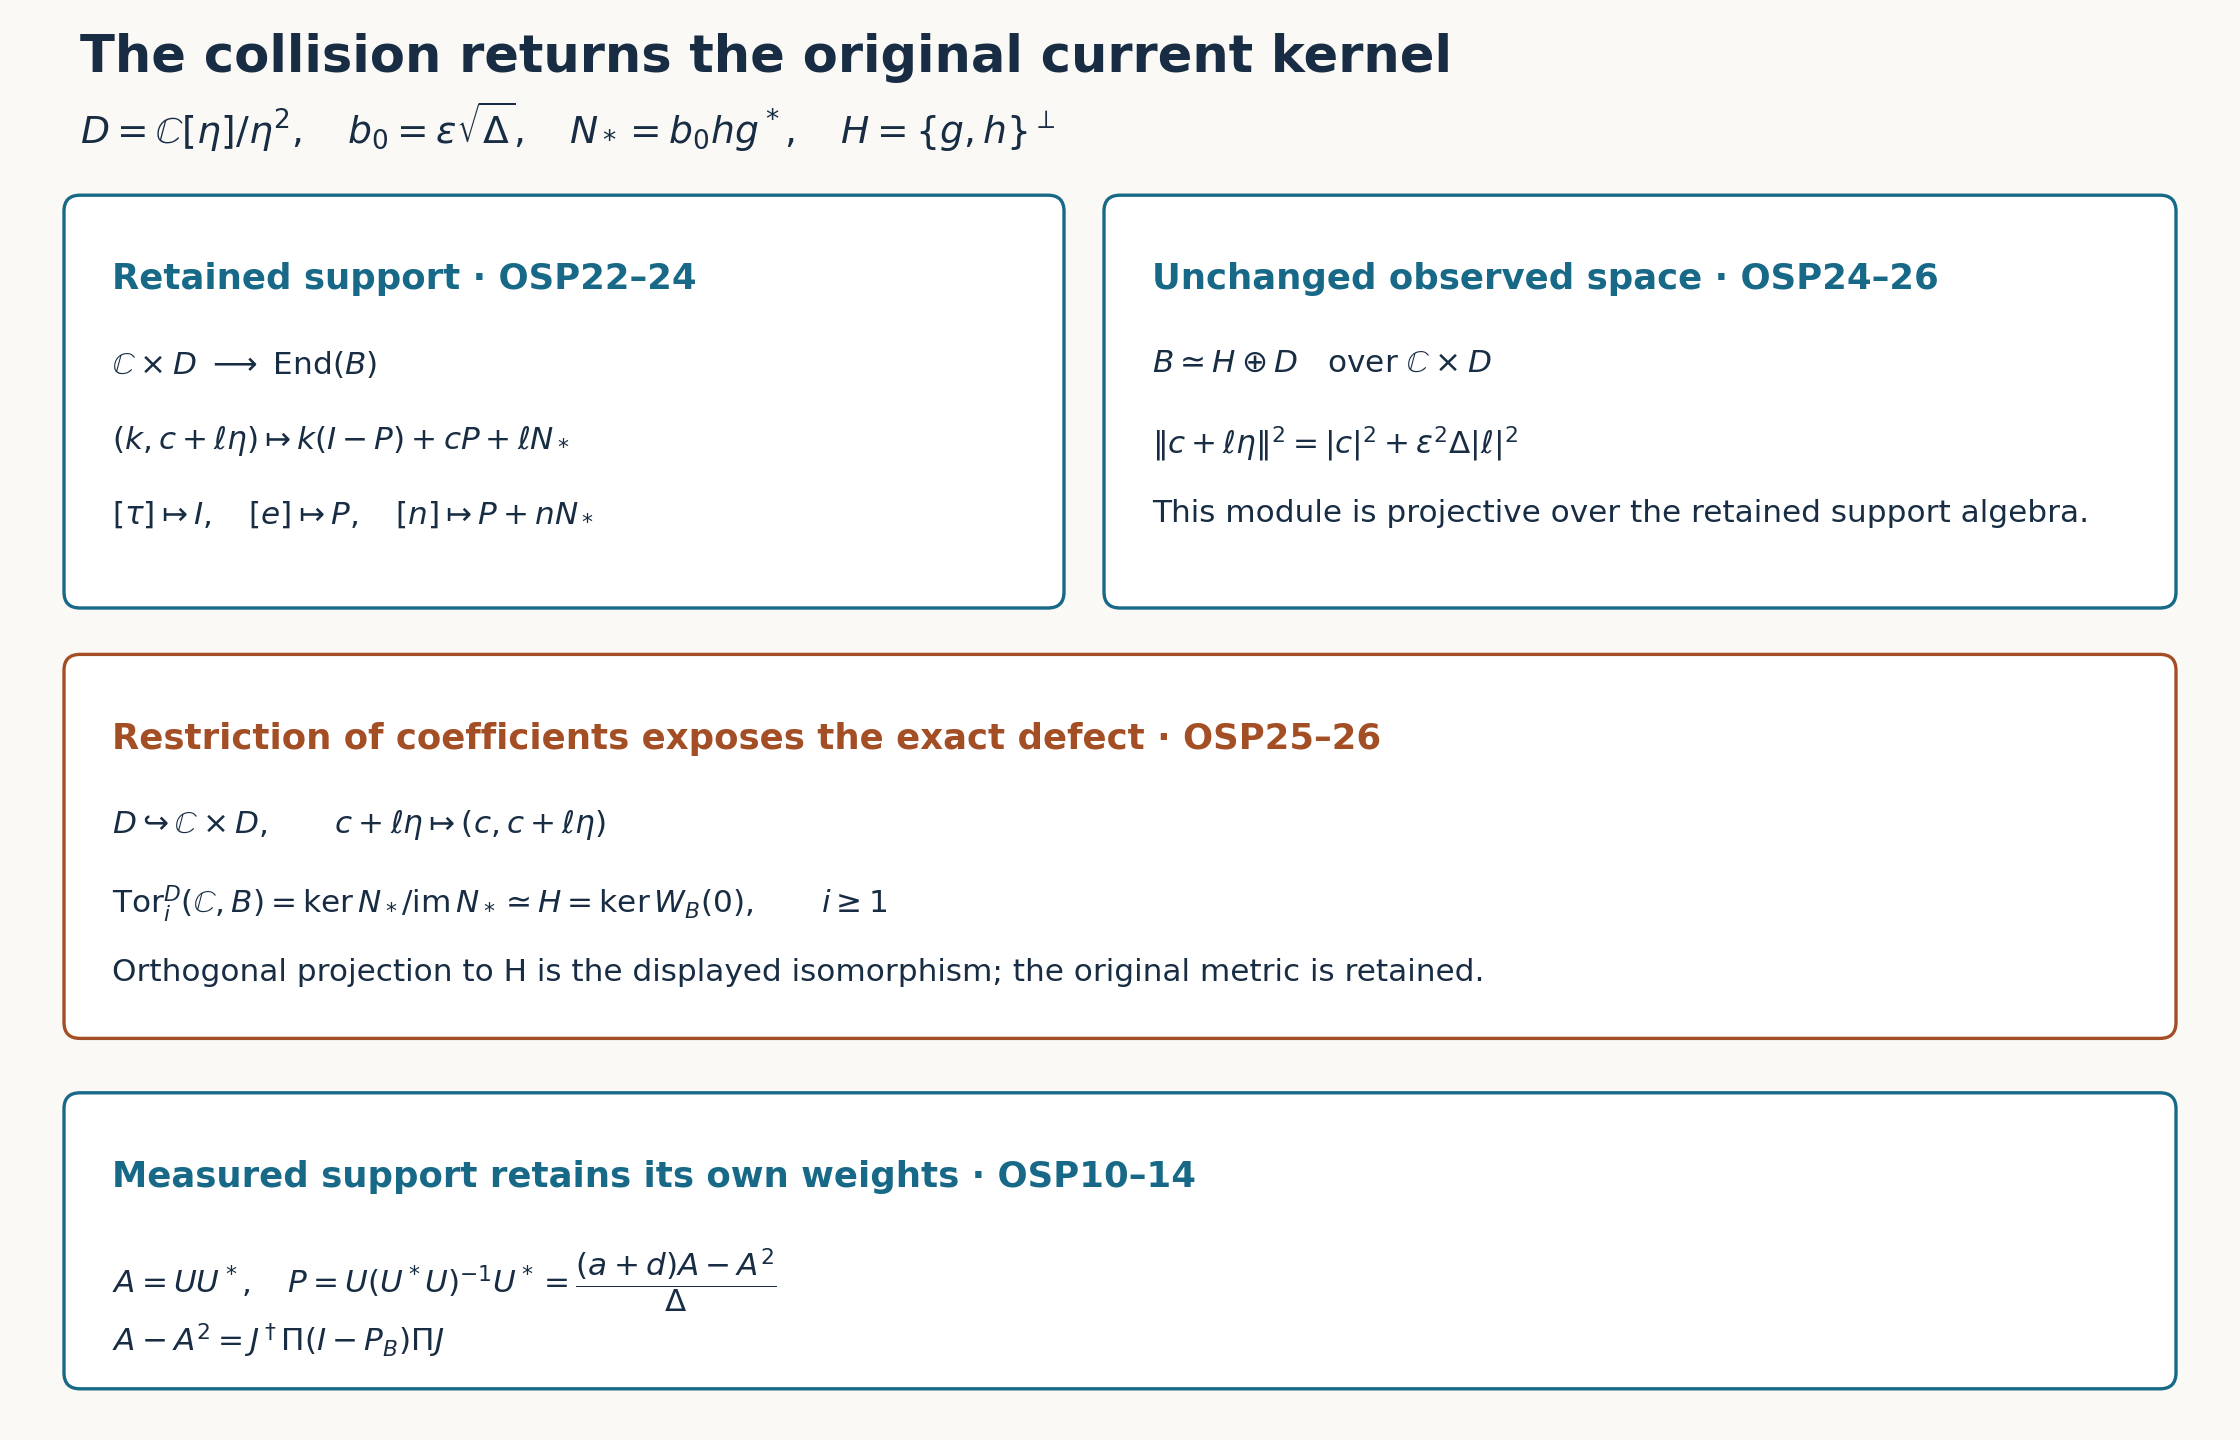
\includegraphics[keepaspectratio,alt={Retained observed support, original-current Tor and measured support}]{figures/19_observed_support.png}}
\caption{Retained observed support, original-current Tor and measured
support}
\end{figure}

The diagram displays OSP22--OSP26 and OSP10--OSP14. Its Delta denotes
the exact Gram determinant mathfrak d; its original support symbol e
denotes the supported integer zero, separately from the metric source
vector bearing that letter in the earlier operator notation. The
complete sharp bound and equality-probe calculations are OSP33--OSP50.
\href{OBSERVED_COLLISION.md}{Observed collision}, OC12--OC17, returns
the same exact perturbation to the characteristic polynomial and inverse
of the full arithmetic operator.

\end{document}
